\section{Implementation of Adaptive Precision and Power Gating}\label{strategy}

\subsection{Power Gating Implementation}

The power gating can be implemented simply by adding PMOS-transistor switches between the functional blocks and the supply voltage \cite{keating_low_2007} as presented in Fig.~\ref{CDS}. 
When the switches are turned off, the corresponding blocks’ current paths will be cut off and thereby the energy is saved. 

It is obvious that the more currents are under control, the more effective the power gating can be. However, to avoid unacceptable IR drop, the total size of the switches may be large, 
and inverters should be inserted between the control signal and the switches’ gates for adequate driving capability. 

Besides, the longer time the blocks can be power gated, the more energy can be saved. And a continuous long time is preferred than separated short time for power gating because
the functional blocks’ recovery speed from power off should also be taken into consideration.
As presented in Fig.~\ref{CDS}, separated short time for power gating will unavoidably waste more
time for the fuctional blocks' recovery 

Therefore, power gating will be efficient for the collumn-parallel ADCs not only due to the large sum of column-parallel currents that can be controled,
but also because that the widely adopted SS conversion logic offers exponential power scaling time.

\begin{figure}[htbp]
	\centerline{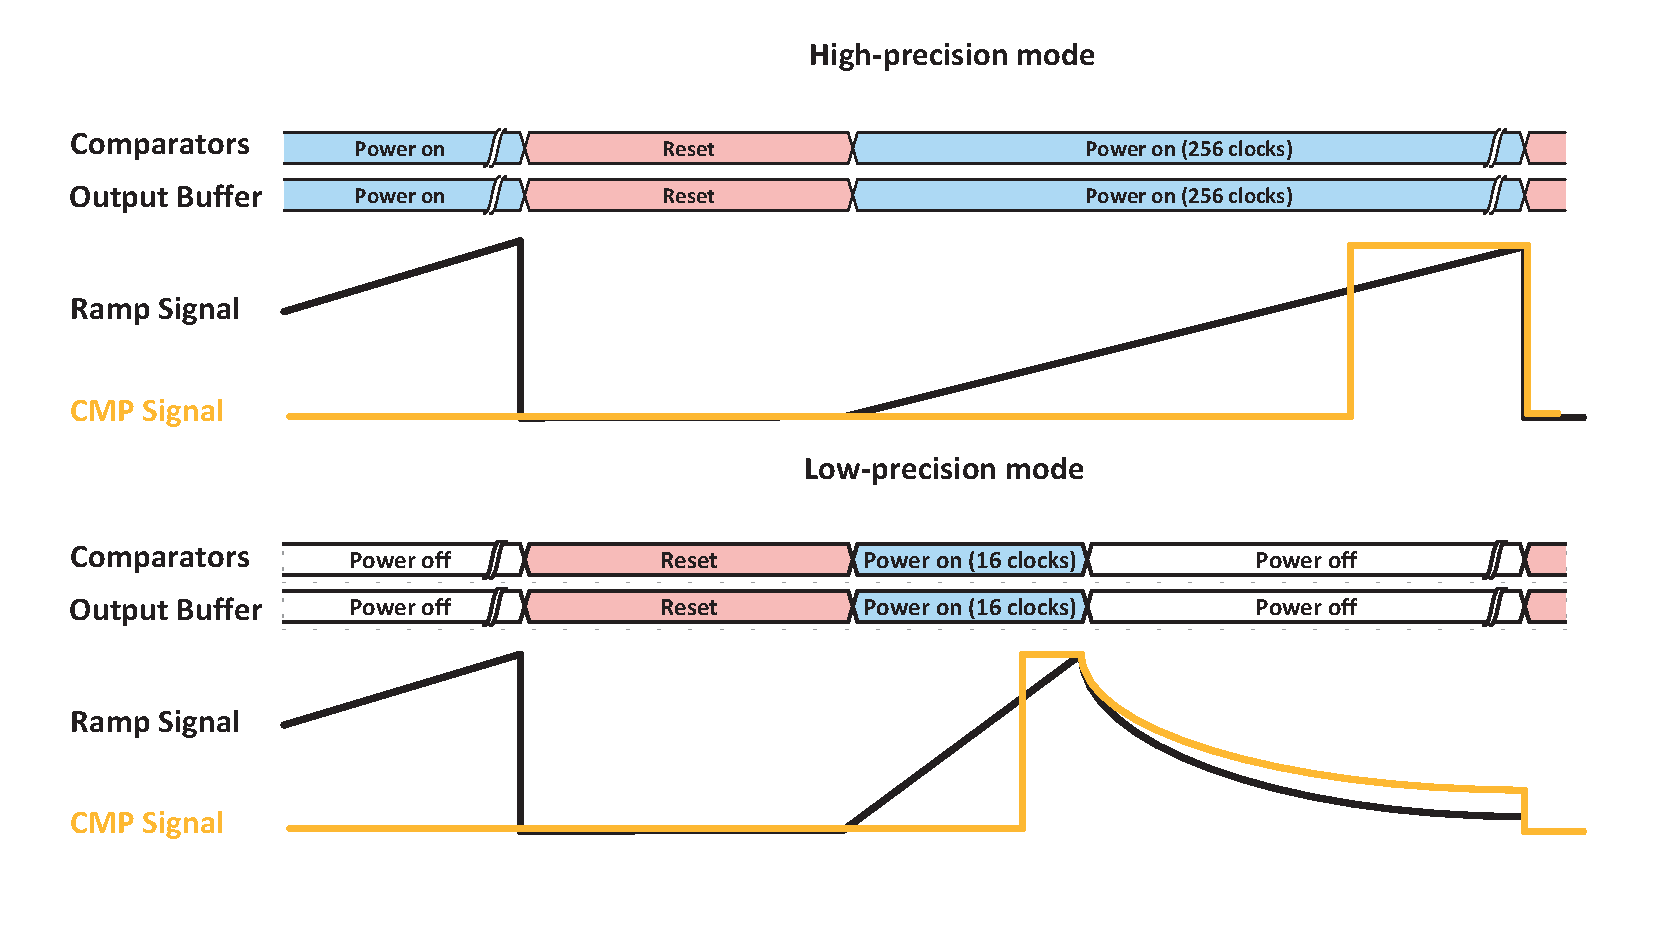
\includegraphics[width=3.5in]{./Figures/SS_pg.eps}}
	\caption{Adaptive Precision and Power Gating Implementation for the SS ADCs.}
	\label{SS_pg}
\end{figure} 

\begin{figure}[htbp]
	\centerline{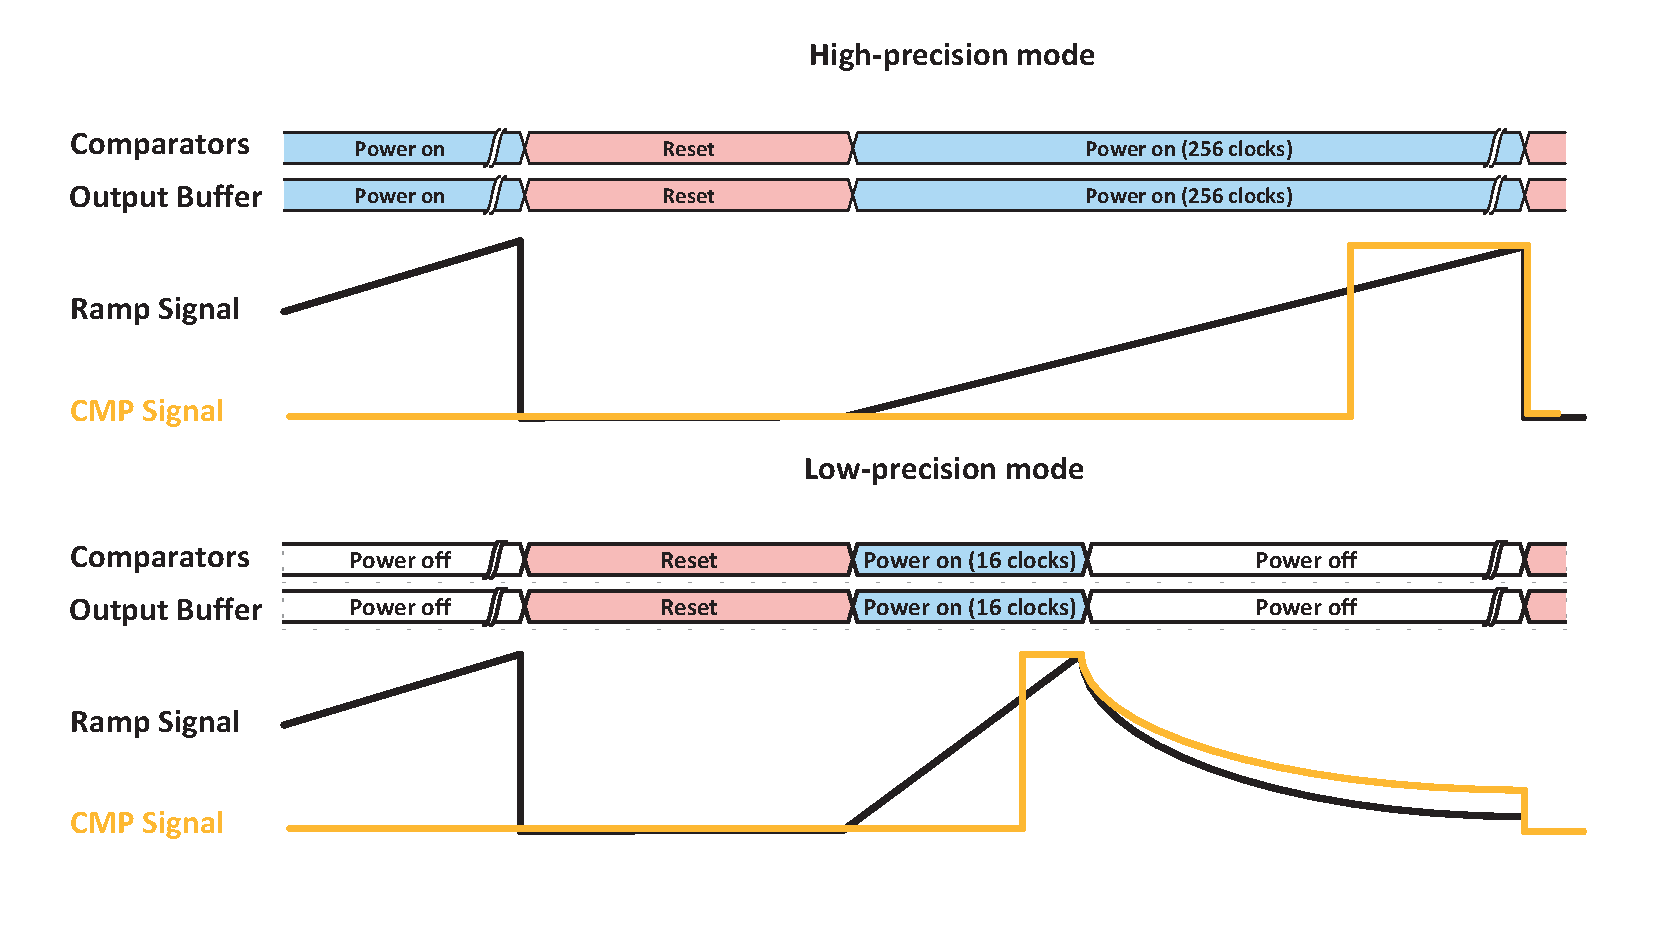
\includegraphics[width=3.5in]{./Figures/SS_pg.eps}}
	\caption{Adaptive Precision and Power Gating Implementation for the SS ADCs.}
	\label{SS_pg}
\end{figure}  

\subsection{Implementation for the SS ADCs}

As evaluated in Sect.~\ref{result}, the SS ADCs’ power consumption is mainly taken up by the column-parallel comparators, bias circuits, and the output buffer of the ramp generator. 
Considering that all bias circuits are settled down only once (tens of microseconds after the whole system's power up) and then other circuits can be settled down quickly by the distributed 
bias circuits, we just apply power gating to the amplifiers in the comparators and the output buffer in the ramp generator.

The related waveform are presented in Fig.~\ref{SS_pg}. For low-precision conversion, the thermometer counter should have been extended to support switching the capacitors in CDAC 16 by 16 
rather than one by one and thereby the ramp signal will reach $V_{refh}$ in 16 steps (for 4 bits) rather than 256 steps (for 8 bits). After the 16 steps the comparators and the output buffer 
can be power gated for a long time, leaving the related signals drop gradually.

To avoid the dropping output signal of comparators causing extra unwanted latch of time information for the low-precision conversion results which should be maintained during the power off time, switches are added to the inverters fowllowing the comparators as presented in Fig.~\ref{CDS}. For power-on conversion, the two inverters' input is connected to the comparator's output, and the two inverter's output will be flipped normally as long as the comparator's output is flipped. During the power-off time, the two inverters' input is connected to the high-level power gating signal which is able to cut off the PMOS-transistor switches for energy saving. And the output signal of the two inverters will keep high-level rather than drop gradually as the comparators' output, preventing the digital latches from being unpredictable enabled and recording the time information incorrectly.

\begin{figure}[htbp]
	\centerline{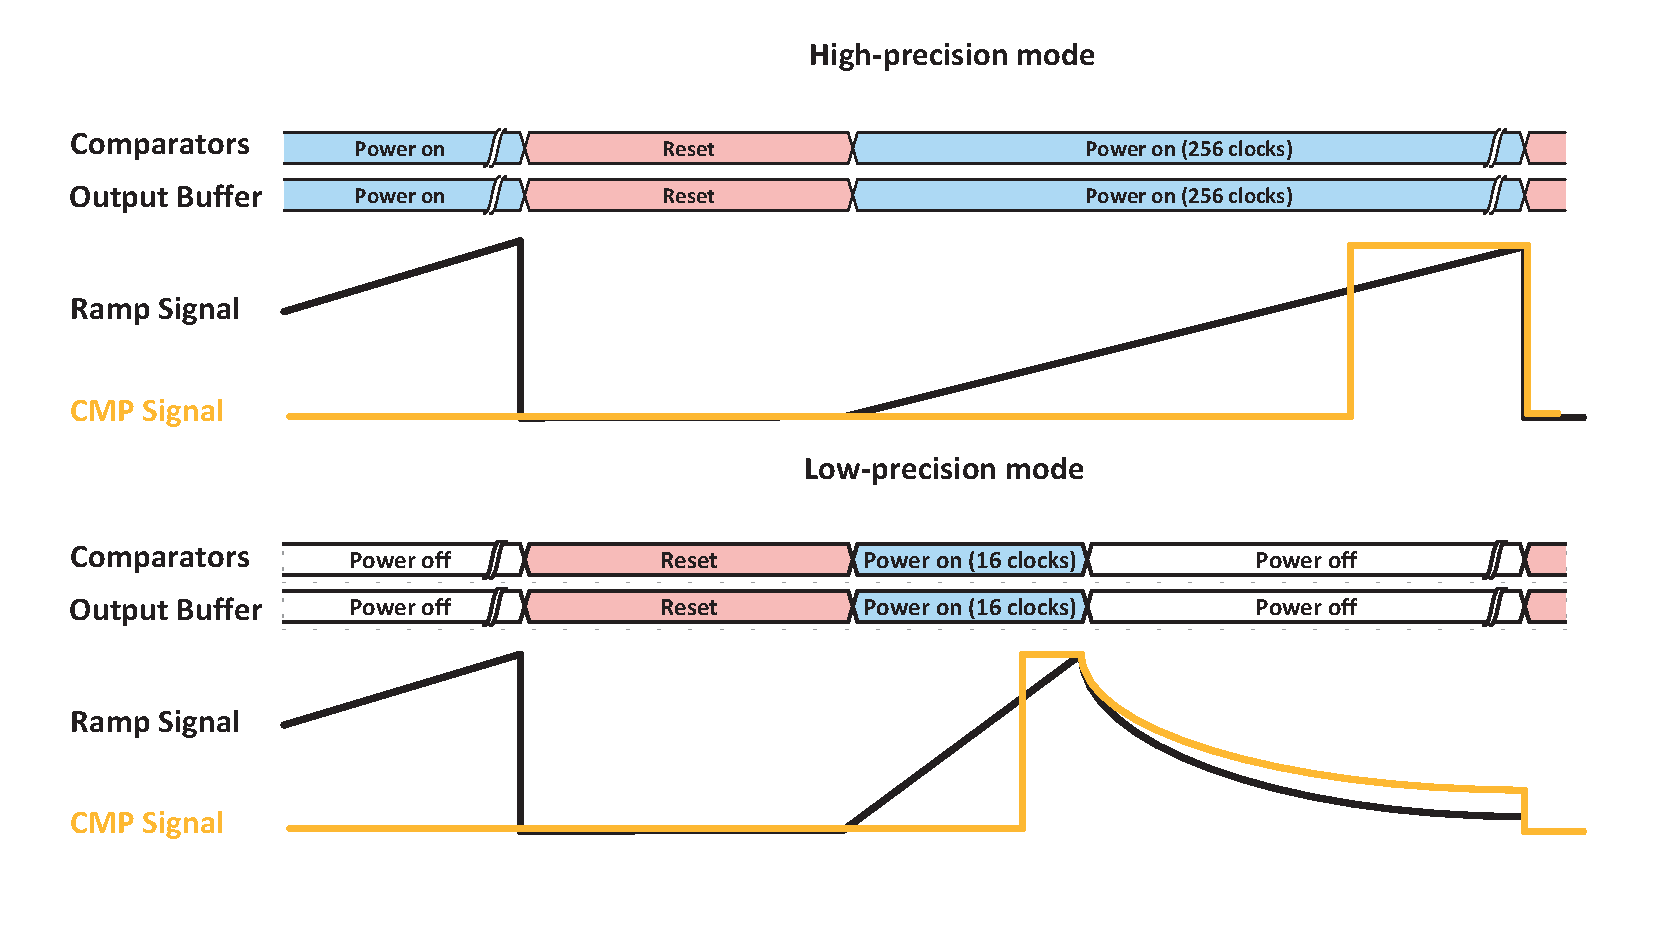
\includegraphics[width=3.5in]{./Figures/SS_pg.eps}}
	\caption{Adaptive Precision and Power Gating Implementation for the SS ADCs.}
	\label{SS_pg}
\end{figure} 

\begin{figure}[htbp]
	\centerline{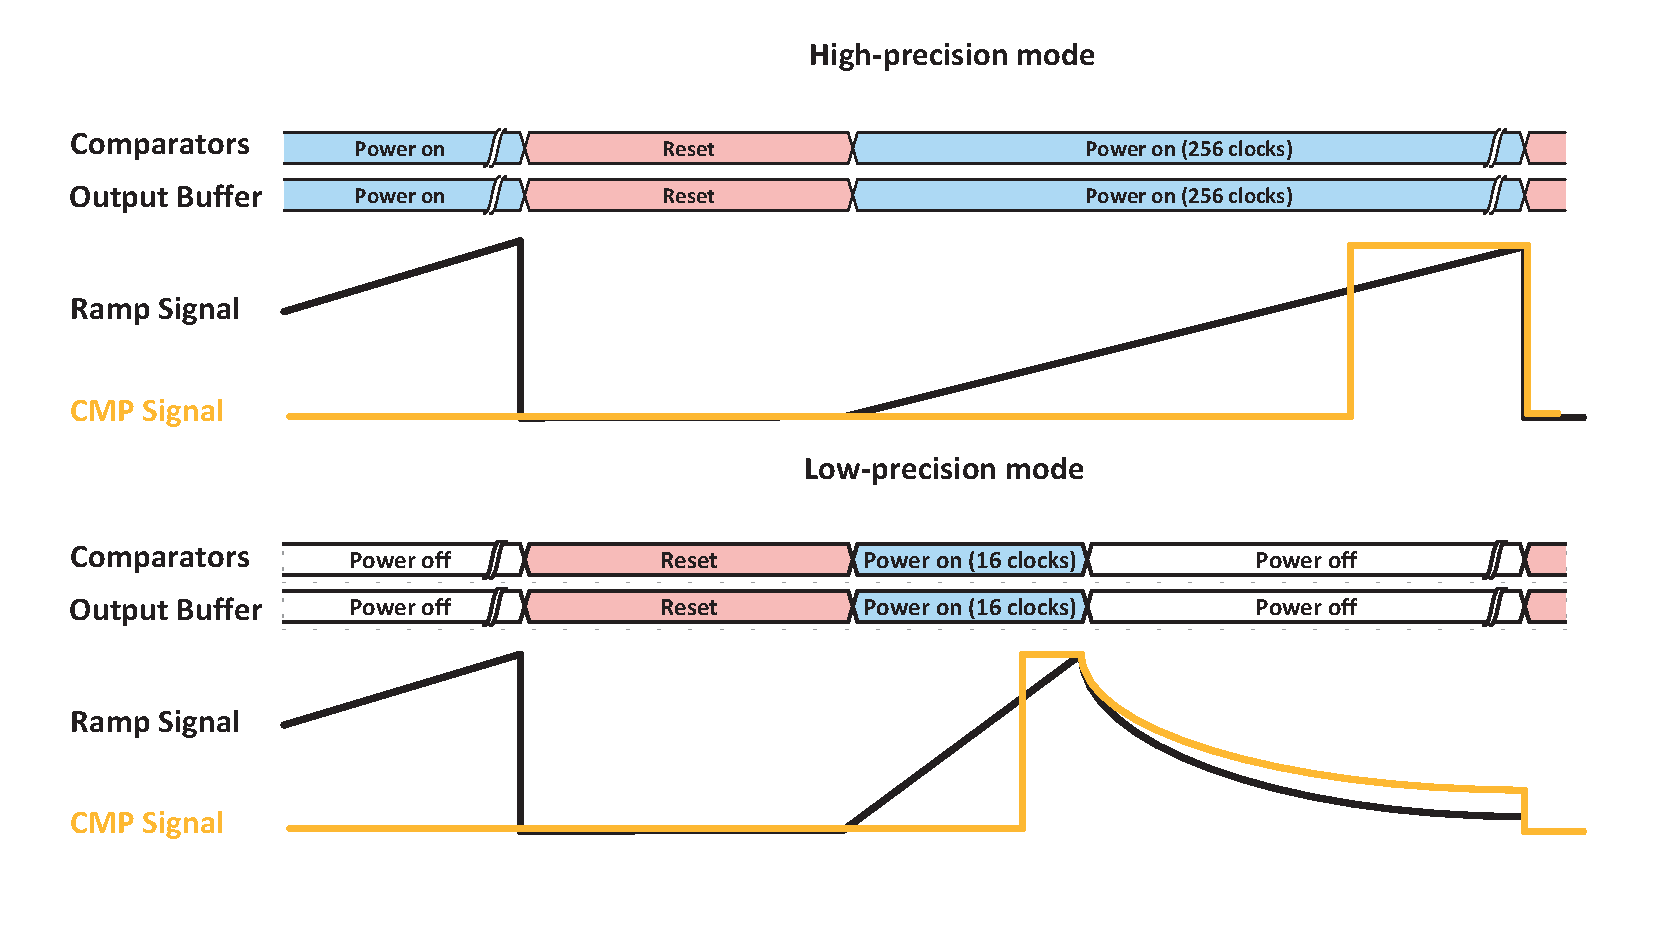
\includegraphics[width=3.5in]{./Figures/SS_pg.eps}}
	\caption{Adaptive Precision and Power Gating Implementation for the SS ADCs.}
	\label{SS_pg}
\end{figure} 

\subsection{Implementation for the SAR/SS ADCs}

As evaluated in Sect.~\ref{result}, the SAR/SS ADCs’ power consumption is mainly taken up by the column-parallel buffers of reference voltages in the SAR sub-ADCs.
It is because that these buffers need to drive relatively large and changing load capacitance, which means relatively large static and dynamical currents are required.
Therefore, gating these buffers will significantly reduce both static power consumption and dynamical power consumption in the ADCs.

The CDS circuits and comparators in the SAR/SS ADCs also consume a certain parts of energy. However, we only choose to take the comparators under control because they can conveniently share the same gating signal as the buffers'. And the gating signal of the buffers can also be consistent with the start signal of the ramp generator. Therefore, gating the buffers and comparators in the SAR/SS ADCs will hardly cost extra control logic but some common-used level-shifters and inverters.

Besides, the power distribution results in Sect.~\ref{result} shows that it is not necessary to take adaptive-precision adjustments inside the ramp generator of the SAR/SS ADCs, making the one-hot counter in the SAR/SS ADCs do not need to support two modes for adaptive-precision.
Therefore, compared with the SS ADCs,  the SAR/SS ADCs relatively require less adaptive-precision adjustments.

The waveform of related signals is presented in Fig.~\ref{SAR_pg}. It is noticed that For low-precison conversion, the ramp signal is generated as usaual but the buffers and comparators will be power off, leaving the 4-bit results converted completely by the SAR logic. 

As for the proportion between the power off time and the conversion time, 64/78 is achieved in the SAR/SS ADCs, which is a little less than the number 240/256 in the SS ADCs. More generally, assuming the low-precision conversion is targeting $a$ bits and the high-presision conversion is targeting $b$ bits, the corresponding equations formulating the proportion of gating time for the SS ADC s and SAR/SS ADCs will be as and , where the $k$ is a coefficient describing how many extra steps are needed for the comparison with SAR logic. Further assuming $k=4$, we can plot the proportion of gating time as in Fig.~\ref{CDS} with different $a$ and $b$ for the SS ADC s and SAR/SS ADCs. It shows that the SS ADCs are suitable for the cases where the $b-a$ are relatively small while the SAR/SS ADCs are able to have better power scaling capability for relatively large $b-a$. On the other hand, the the SS ADCs oringinally have trouble converting higher than 10 bits for full-precision because exponential increasing conversion steps will limit the throuput. Therefore, adopting SS ADCs for 4/8 adaptive-precision and SAR/SS ADCs for 4/10 adaptive-precision takes advantages and avoid weaknesses of the two different achitecture, respectively.

\begin{figure}[htbp]
	\centerline{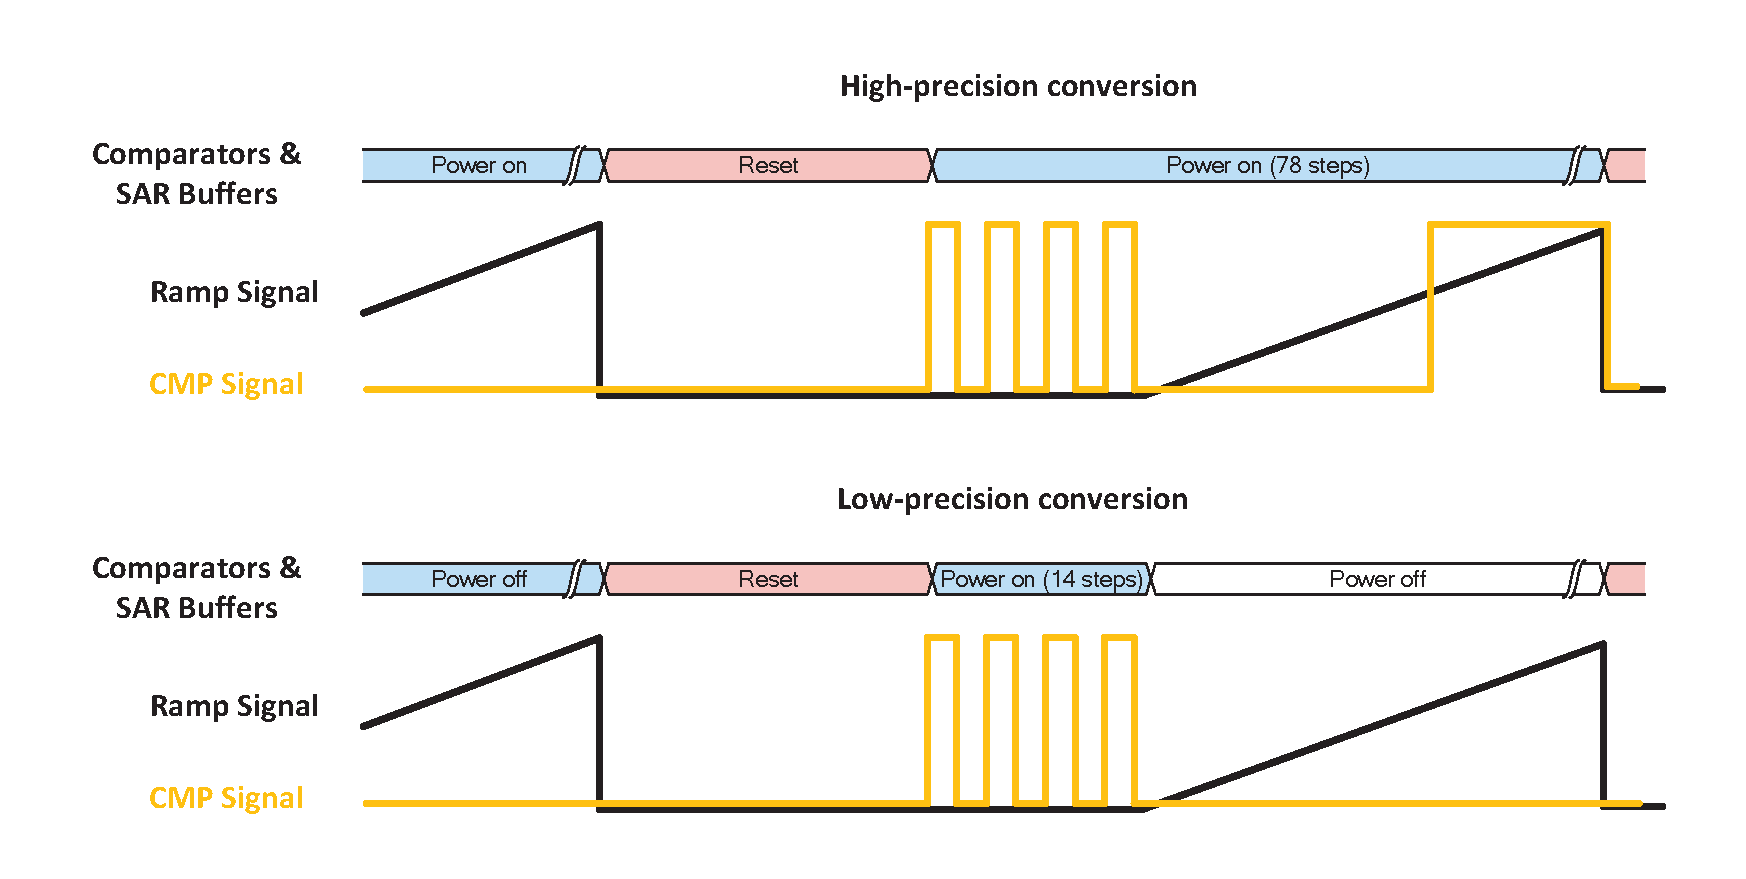
\includegraphics[width=3.5in]{./Figures/SAR_pg.eps}}
	\caption{Adaptive Precision and Power Gating Implementation for the SAR/SS ADCs.}
	\label{SAR_pg}
\end{figure} 